\documentclass[aspectratio=169]{beamer}
\usepackage{color,amsmath}
\usepackage{subfigure}
\usepackage{booktabs}
\usepackage{framed}
\usepackage{comment}
\usepackage{url}


%%%%%%%%%%%%%%%%%%%%%%%%%%
\title[]{Introduction to group activity}
\author[]{Matthew J. Salganik\\Department of Sociology\\Princeton University}
\date[]{Summer Institute in Computational Social Science\\June 21, 2018
\vfill
\begin{flushleft}
{\scriptsize
The Summer Institute in Computational Social Science is supported by grants from the Russell Sage Foundation and the Alfred P. Sloan Foundation.}
\end{flushleft}
\begin{flushright}

\includegraphics[width=0.1\textwidth]{figures/cc-by.png}
\end{flushright}
}
\begin{document}
%%%%%%%%%%%%%%%%%%%%%%%%%%
\frame{\titlepage}
%%%%%%%%%%%%%%%%%%%%%%%%%%
\begin{frame}

\begin{center}
\only<1>{
\includegraphics[width=0.9\textwidth]{figures/goel_online_2017_title}}
\only<2>{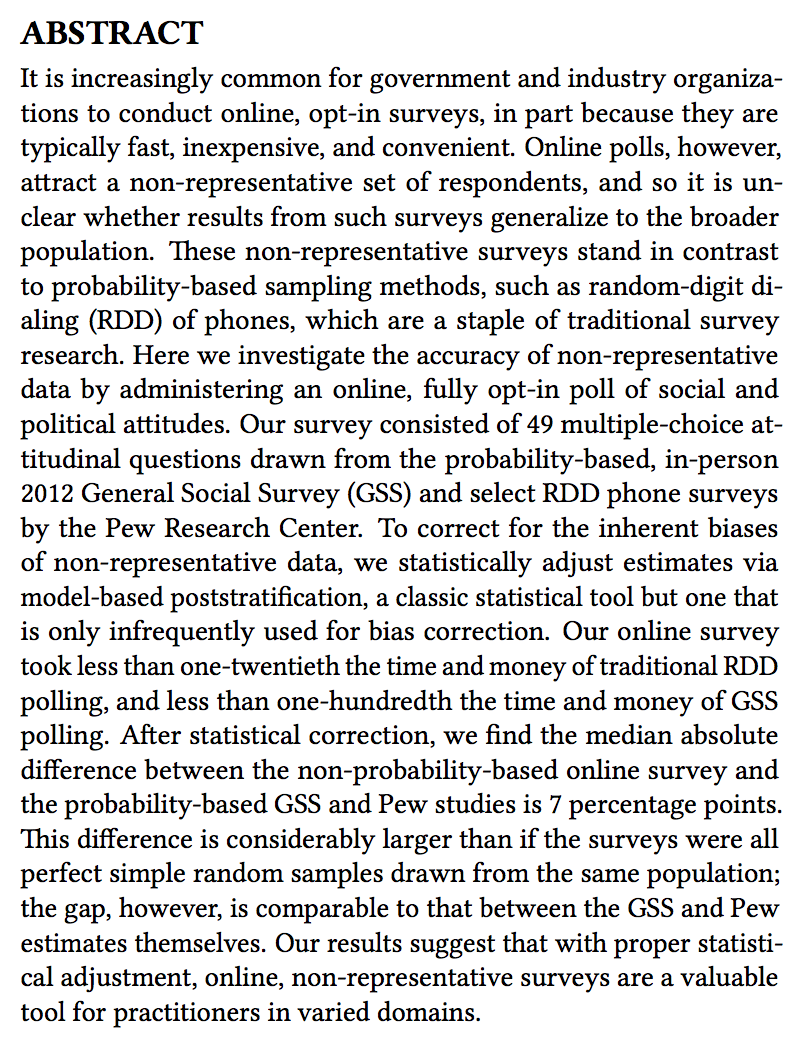
\includegraphics[width=0.4\textwidth]{figures/goel_online_2017_abstract}}
\end{center}

\vfill
\url{https://5harad.com/papers/dirtysurveys.pdf}

\end{frame}
%%%%%%%%%%%%%%%%%%%%%%%%%%%
\begin{frame}

Activity:
\begin{itemize}
\item Design a questionaire using questions already asked on high quality surveys
\pause
\item Recruit participants from Amazon Mechanical Turk and have them complete your questionnaire  
\pause
\item Compare results from your survey to the results from the high-quality survey
\pause
\item Try different approaches to weighting and see how the change the estimates
\pause
\item De-identify and open-source data 
\end{itemize}

\end{frame}
%%%%%%%%%%%%%%%%%%%%%%%%%%
\begin{frame}

This activity will give you practice:
\begin{itemize}
\item Collecting survey data
\pause
\item Analyzing survey data (data wrangling and post-stratification)
\pause
\item Working with Amazon Mechanical Turk
\pause
\item Archiving data for other researchers
\end{itemize}

\vfill
Remember: This is a learning activity so try whatever you want.

\end{frame}
%%%%%%%%%%%%%%%%%%%%%%%%%%%
\begin{frame}

Our recommended work flow:
\begin{itemize}
\item Create survey on Google Forms
\item Deploy to MTurk
\item Take a break
\end{itemize}

\end{frame}
%%%%%%%%%%%%%%%%%%%%%%%%%%
\begin{frame}

\begin{center}
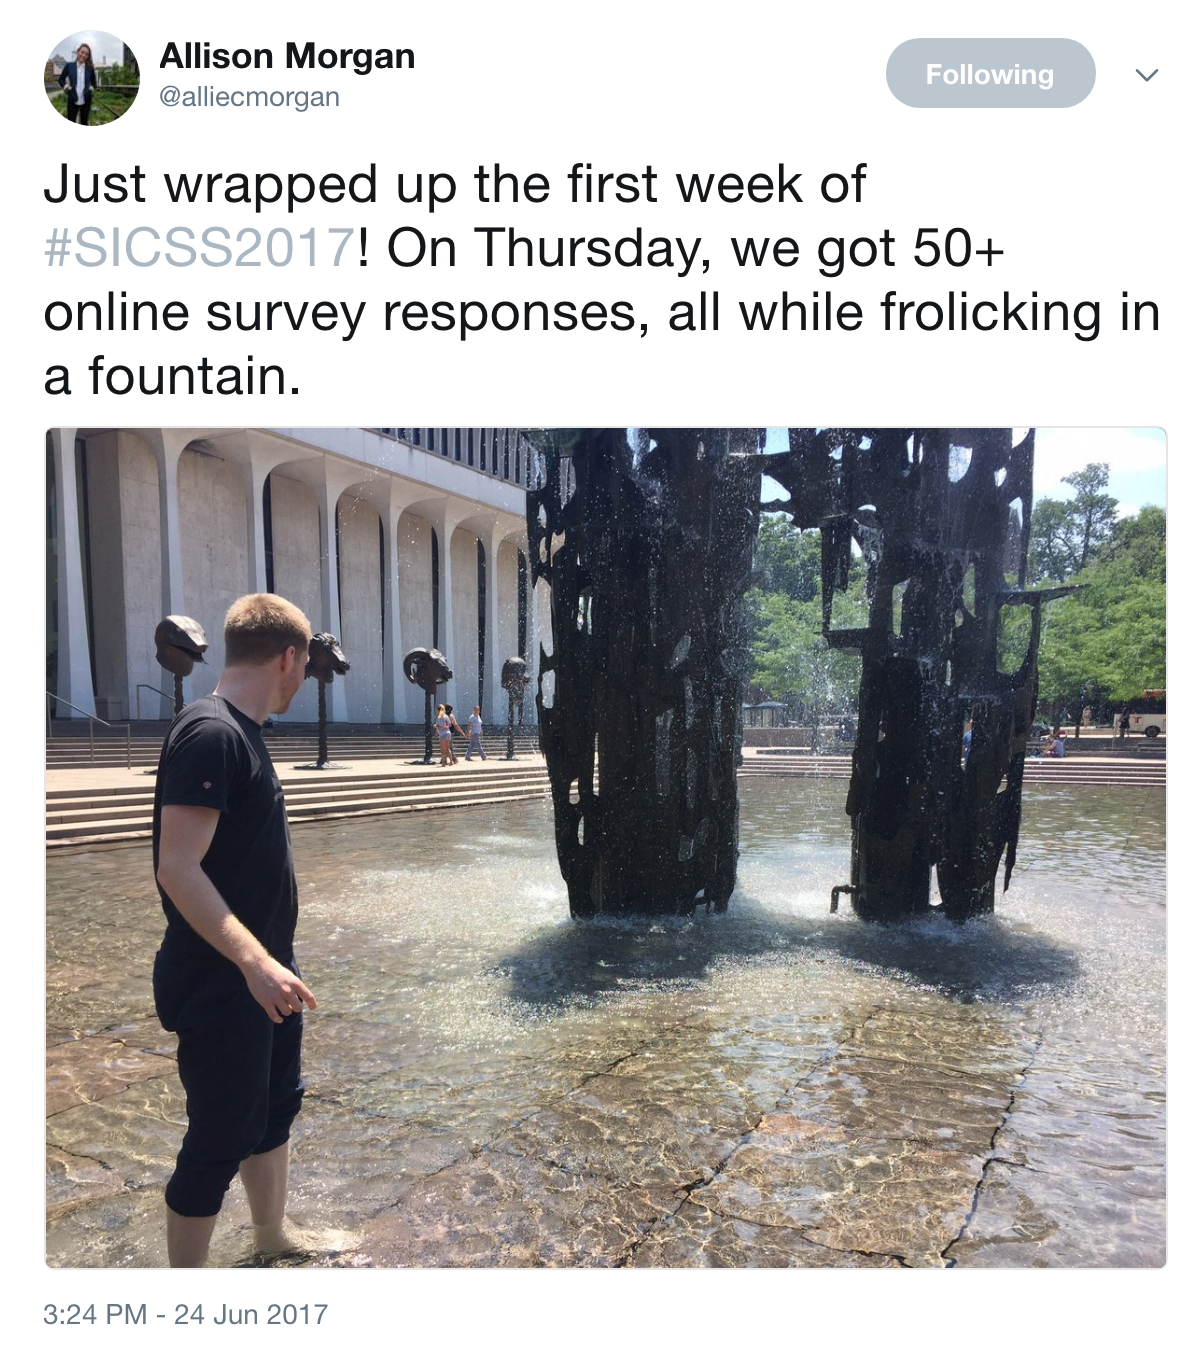
\includegraphics[width=0.4\textwidth]{figures/morgan_tweet}
\end{center}

\end{frame}
%%%%%%%%%%%%%%%%%%%%%%%%%%
\begin{frame}

Our recommended work flow:
\begin{itemize}
\item Create survey on Google Forms
\item Deploy to MTurk
\item Take a break
\item Validate and pay workers
\item Analyze the much larger sample that we have collected for you
\item De-identify and open-source the data that you collected
\end{itemize}

\end{frame}
%%%%%%%%%%%%%%%%%%%%%%%%%%

\end{document}
